% Created 2020-07-02 jue 08:13
% Intended LaTeX compiler: pdflatex
\documentclass[presentation,aspectratio=169]{beamer}
\usepackage[utf8]{inputenc}
\usepackage[T1]{fontenc}
\usepackage{graphicx}
\usepackage{grffile}
\usepackage{longtable}
\usepackage{wrapfig}
\usepackage{rotating}
\usepackage[normalem]{ulem}
\usepackage{amsmath}
\usepackage{textcomp}
\usepackage{amssymb}
\usepackage{capt-of}
\usepackage{hyperref}
\usepackage{khpreamble}
\usepackage{amssymb}
\usepgfplotslibrary{groupplots}
\DeclareMathOperator{\shift}{q}
\DeclareMathOperator{\diff}{p}
\usetheme{default}
\author{Kjartan Halvorsen}
\date{2020-07-01}
\title{Control Computarizado - Muestreo y el efecto de alias}
\hypersetup{
 pdfauthor={Kjartan Halvorsen},
 pdftitle={Control Computarizado - Muestreo y el efecto de alias},
 pdfkeywords={},
 pdfsubject={},
 pdfcreator={Emacs 26.3 (Org mode 9.3.6)}, 
 pdflang={English}}
\begin{document}

\maketitle

\section{Intro}
\label{sec:org2fb97dc}

\begin{frame}[label={sec:orgc9075c2}]{Sistemas híbridas}
\begin{center}
\includegraphics[width=0.7\linewidth]{../../figures/fig7-2.png}
\end{center}
\end{frame}

\section{El teorema del muestro}
\label{sec:orge4338df}
\begin{frame}[label={sec:orgb226ed7}]{Retos en control computarizado - fenómeno de alias}
\begin{columns}
\begin{column}{0.6\columnwidth}
\begin{center}
  \begin{tikzpicture}
    \node {\includegraphics[width=0.99\linewidth]{../../figures/comp-contr-sys.png}};
    \node[pin=145:{60Hz mains hum}] at (2.7,2.4) {};
    \node[pin=-60:{90Hz sampling freq}] at (0.5,-1.4) {};
  \end{tikzpicture}
\end{center}
\end{column}
\begin{column}{0.4\columnwidth}
\includegraphics[width=0.99\linewidth]{../../figures/aliasing-example-60Hz}
\end{column}
\end{columns}
\end{frame}

\begin{frame}[label={sec:orgdd65142}]{Efecto de alias en imágenes}
\begin{center}
\includegraphics[width=0.45\linewidth]{../../figures/Moire_pattern_of_bricks.png}
\includegraphics[width=0.45\linewidth]{../../figures/Moire_pattern_of_bricks_small.png}
\end{center}
\end{frame}

\begin{frame}[label={sec:org6963b84}]{El teorema del muestreo}
Shannon y Nyquist:

Una señal continua cuya transformada de Fourier es cero fuera del intervalo \((-\omega_0, \omega_0)\)  puede ser reconstruido completamente usando valores (muestros) equidistantes de la señal, siempre cuando la frecuencia de muestreo sea por lo menos \(2\omega_0\). 

\begin{center}
  \begin{tikzpicture}[scale=1.2]
    \draw[->] (-3,0) -- (3,0) node[below] {$\omega$};
    \draw[->] (0,0) -- (0,1.5);
    \draw[red, thick] (0,1) to (1,0);
    \draw[red, thick] (0,1) to (-1,0);
    \node at (1,-0.3) {$\omega_0$};
    \node at (-1,-0.3) {$-\omega_0$};
    \node at (0,-0.3) {$0$};
    \node[coordinate, pin=-90:{$2\omega_0$}] at (2,0) {};

  \end{tikzpicture}
\end{center}
\end{frame}

\begin{frame}[label={sec:orgcb4d390}]{Un modelo del muestreo}
Una señal muestreada tiene una representación en tiempo continuo usando el modelo de modulación por un \alert{tren de impulsos}
\begin{center}
\(m(t) = \sum_{k=-\infty}^{\infty} \delta(t-kh)\)\hspace*{10mm}
 \includegraphics[width=0.4\linewidth]{../../../figures/modulation-model-blocks}
\end{center}

\[f_s(t) = f(t)m(t) = f(t) \sum_{k=-\infty}^{\infty} \delta(t-kh) = \sum_{k=-\infty}^{\infty} f(t)\delta(t-kh) = \sum_{k=-\infty}^{\infty} f(kh) \delta(t-kh) \]


\begin{center}
\includegraphics[width=0.8\linewidth]{../../figures/modulation-model-timeseries}
\end{center}
\end{frame}

\begin{frame}[label={sec:org8b19f69}]{Transformada de Fourier de la señal muestreada}
La relación entre la transformada de la señal continua \(f(t)\) y la de su versión muestreada \(f_s(t)\):

\[ F_s(\omega) = \frac{1}{h} \sum_n F(\omega + n\omega_s) \]

\begin{columns}
\begin{column}{0.5\columnwidth}
\(F_s(\omega)\) se obtiene sumando repeticiones de \(F(\omega)\) en cada múltiple de la frecuencia de muestro \(\omega_s\). Esta es la causa del fenómeno de \alert{alias} y la distorsión conocido como \alert{plegado de frecuencia} (\emph{frequency folding}).
\end{column}

\begin{column}{0.5\columnwidth}
\begin{center}
\includegraphics[width=0.68\linewidth]{../../figures/frequency-folding.png}
\end{center}
\end{column}
\end{columns}
\end{frame}

\section{Exercises using line spectra}
\label{sec:org3e82c3a}
\begin{frame}[label={sec:org03738b6}]{Transformada de Fourier de un exponencial complejo}
La función  \(x(t) = \mathrm{e}^{i\omega_1 t}\) 
\begin{center}
  \begin{tikzpicture}[scale=2]
    \draw[->] (-1.2, 0) -- (1.2,0) node[below] {Re};
    \draw[->] (0, -1.2) -- (0,1.2) node[left] {Im};
    \draw[domain=0:360, samples=361, dashed] plot ({cos(\x)}, {sin(\x)});
    \node[circle, fill, inner sep=2pt, red] (pnt) at (0.868, 0.5) {};
    \draw[dashed, blue] (0,0) to (0.868, 0.5);
    \draw[domain=0:30, samples=20, ->] plot ({0.6*cos(\x)}, {0.6*sin(\x)});
    \node at (0.7, 0.2) {$\omega_1 t$};
    \node[pin=-135:{1}, coordinate] at (1, 0) {};
    \node[right of=pnt, node distance=3mm, anchor=west] {$x(t) = \mathrm{e}^{i\omega_1 t} = \cos(\omega_1 t) + i\sin(\omega_1 t)$};
  \end{tikzpicture}
\end{center}
tiene la transformada de Fourier
\[X(\omega) = \int_{-\infty}^{\infty} x(t) \mathrm{e}^{-i\omega t}dt = \int_{-\infty}^{\infty} \mathrm{e}^{i(\omega_1 - \omega) t}dt = \delta(\omega_1 - \omega)\] 
\end{frame}

\begin{frame}[label={sec:org6fe2bdd}]{Transformada de Fourier de una sinusoide}
Una sinusoide \(y(t) = \sin(\omega_1 t)\) tiene toda su energía concentrada en una sola frecuencia, \(\omega=\unit{\omega_1}{rad\per\second}\). 
\begin{center}
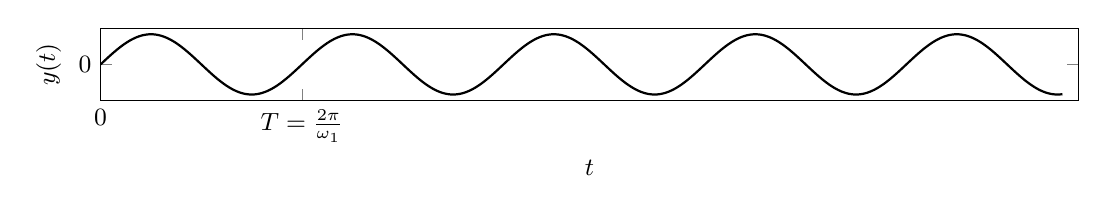
\begin{tikzpicture}
\small
\pgfmathsetmacro{\ww}{1}
\pgfmathsetmacro{\TT}{2*pi/\ww}
\begin{axis}[
width=14cm,
height=2.5cm,
xlabel={$t$},
ylabel={$y(t)$},
xmin=0.,
xmax=30.5,
ytick = {0},
xtick = {0, \TT},
xticklabels={0, $T=\frac{2\pi}{\omega_1}$},
]
\addplot+[black, thick,no marks, domain=0:30, samples=400,variable=t] { sin(deg(\ww*t)) };
\end{axis}
\end{tikzpicture}
\end{center}
Dado de que \[y(t) = \sin(\omega_1 t) = \frac{1}{2i} \left( \mathrm{e}^{i\omega_1 t} - \mathrm{e}^{-i \omega_1 t} \right)\]
la transformada de Fourier es
\[ Y(\omega) = \frac{1}{2i} \left( \delta(\omega_1 - \omega) - \delta(\omega_1 + \omega) \right)\]
\end{frame}

\begin{frame}[label={sec:orgedb794a}]{Ejercicio 1: La transformada de Fourier de una sinusoide}
Considera la siguiente señal

\begin{center}
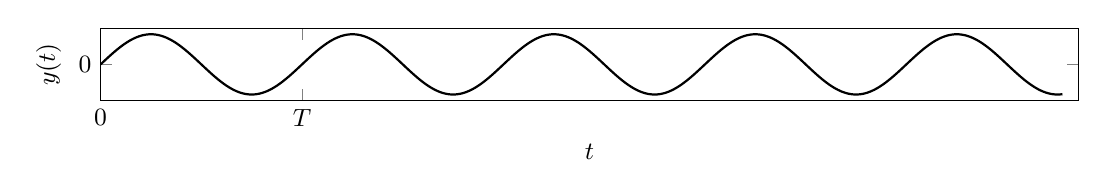
\begin{tikzpicture}
\small
\pgfmathsetmacro{\ww}{1}
\pgfmathsetmacro{\TT}{2*pi/\ww}
\begin{axis}[
width=14cm,
height=2.5cm,
xlabel={$t$},
ylabel={$y(t)$},
xmin=0.,
xmax=30.5,
ytick = {0},
xtick = {0, \TT},
xticklabels={0, $T$},
]
\addplot+[black, thick,no marks, domain=0:30, samples=400,variable=t] { sin(deg(\ww*t)) };
\end{axis}
\end{tikzpicture}
\end{center}

Cuál de los espectros abajo (\(|Y(i\omega)|\)) corresponde a la señal?


\pgfplotsset{
dirac/.style={
mark=triangle*,
mark options={scale=0.6},
ycomb,
scatter,
visualization depends on={y/abs(y)-1 \as \sign},
scatter/@pre marker code/.code={\scope[rotate=90*\sign,yshift=-2pt]}
}
}
  \begin{tikzpicture}
  \footnotesize

  \pgfmathsetmacro{\ww}{1}
  \pgfmathsetmacro{\TT}{2*pi/\ww}
  \pgfmathsetmacro{\omegaone}{2/\TT}
  \pgfmathsetmacro{\omegatwo}{pi/\TT}
  \pgfmathsetmacro{\omegathree}{1/\TT}
  \pgfmathsetmacro{\omegafour}{2*pi/\TT}

  \begin{groupplot}[group style={group size=2 by 2, vertical sep=1.2cm, horizontal sep=1.3cm},
  width=7cm,
  height=2.5cm,
  xlabel={$\omega$ [rad/s]},
  ylabel={$|Y(i\omega)|$},
  xmin=-1.5,
  xmax=1.5,
  ytick = \empty,
  xtick = \empty,
  ]
  \nextgroupplot[xtick={-\omegaone, 0, \omegaone}, 
  xticklabels={$-\frac{2}{T}$, 0, $\frac{2}{T}$}]
  \addplot[red, thick, dirac] coordinates {(-\omegaone, 1) (\omegaone, 1)};

  \nextgroupplot[xtick={-\omegatwo, 0, \omegatwo}, 
  xticklabels={$-\frac{\pi}{T}$, 0, $\frac{\pi}{T}$}]
  \addplot[red, thick, dirac] coordinates {(-\omegatwo, 1) (\omegatwo, 1)};

  \nextgroupplot[xtick={-\omegathree, 0, \omegathree}, 
  xticklabels={$-\frac{1}{T}$, 0, $\frac{1}{T}$}]
  \addplot[red, thick, dirac] coordinates {(-\omegathree, 1) (\omegathree, 1)};

  \nextgroupplot[xtick={-\omegafour, 0, \omegafour}, 
  xticklabels={$-\frac{2\pi}{T}$, 0, $\frac{2\pi}{T}$}]
  \addplot[red, thick, dirac] coordinates {(-\omegafour, 1) (\omegafour, 1)};
  \end{groupplot}

  \node[red] at (group c1r1.center) {\huge 1};
  \node[red] at (group c2r1.center) {\huge 2};
  \node[red] at (group c1r2.center) {\huge 3};
  \node[red] at (group c2r2.center) {\huge 4};
  \end{tikzpicture}
\end{frame}
\begin{frame}[label={sec:org9c9ef9c}]{Ejercicio 2: Dos sinusoides}
Considera una señal con la siguiente transformada de Fourier

\pgfplotsset{
dirac/.style={
mark=triangle*,
mark options={scale=0.6},
ycomb,
scatter,
visualization depends on={y/abs(y)-1 \as \sign},
scatter/@pre marker code/.code={\scope[rotate=90*\sign,yshift=-2pt]}
}}
\begin{center}
\begin{tikzpicture}
\small
\pgfmathsetmacro{\wwone}{1}
\pgfmathsetmacro{\wwtwo}{5*\wwone}
\begin{axis}[
width=14cm,
height=2.5cm,
xlabel={$\omega$ [rad/s]},
ylabel={$|Y(i\omega)|$},
xmin=-7,
xmax=7,
ymin=-0.5,
ytick=\empty,
xtick = {-\wwtwo, -\wwone, 0, \wwone, \wwtwo},
% ticklabels={$-5\omega_1$, $-\omega_1$, 0, $\omega_1$, $5\omega_1$},
]
\addplot[black, thick, dirac] coordinates {(-\wwtwo, 0.3) (-\wwone, 1) (\wwone, 1) (\wwtwo, 0.3)};
\end{axis}
\end{tikzpicture}
\end{center}

Cuál de las señales abajo corresponde a la transformada de Fourier arriba?


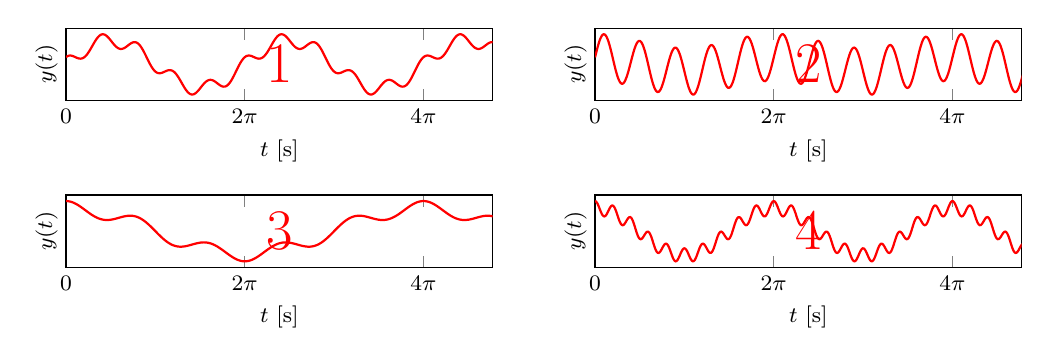
\begin{tikzpicture}
\footnotesize

\pgfmathsetmacro{\wwone}{1}
\pgfmathsetmacro{\wwtwo}{5*\wwone}

\begin{groupplot}[group style={group size=2 by 2, vertical sep=1.2cm, horizontal sep=1.3cm},
width=7cm,
height=2.5cm,
xlabel={$t$ [s]},
ylabel={$y(t)$},
xmin=0,
xmax=15,
ytick = \empty,
xtick = \empty,
domain=0:20,
samples=600,
variable=t,
]

\nextgroupplot[xtick={0, 6.28, 12.56}, xticklabels={0, $2\pi$, $4\pi$},]
 \addplot[red, thick, no marks] { sin(deg(\wwone*t)) + 0.3*cos(deg(\wwtwo*t))};

\nextgroupplot[xtick={0, 6.28, 12.56}, xticklabels={0, $2\pi$, $4\pi$},]
 \addplot[red, thick, no marks] { 0.3*cos(deg(\wwone*t)) + sin(deg(\wwtwo*t))};

\nextgroupplot[xtick={0, 6.28, 12.56}, xticklabels={0, $2\pi$, $4\pi$},]
 \addplot[red, thick, no marks] { cos(deg(0.5*\wwone*t)) + 0.3*cos(deg(0.5*\wwtwo*t))};

\nextgroupplot[xtick={0, 6.28, 12.56}, xticklabels={0, $2\pi$, $4\pi$},]
 \addplot[red, thick, no marks] { cos(deg(\wwone*t)) + 0.3*cos(deg(2*\wwtwo*t))};

\end{groupplot}

\node[red] at (group c1r1.center) {\huge 1};
\node[red] at (group c2r1.center) {\huge 2};
\node[red] at (group c1r2.center) {\huge 3};
\node[red] at (group c2r2.center) {\huge 4};
\end{tikzpicture}
\end{frame}
\begin{frame}[label={sec:orgc6b69ff}]{Ejercicio 3: Transformada de Fourier de una sinusoide muestreada}
La figura siguiente enseña una sinusoide con periodo \(T\) y su versión muestreada con period de muestreo \(h=\frac{2}{3}T\).


 \pgfplotsset{
dirac/.style={
mark=triangle*,
mark options={scale=0.6},
ycomb,
scatter,
visualization depends on={y/abs(y)-1 \as \sign},
scatter/@pre marker code/.code={\scope[rotate=90*\sign,yshift=-2pt]}
}
}
\begin{center}
\begin{tikzpicture}
\small
\pgfmathsetmacro{\ww}{1}
\pgfmathsetmacro{\TT}{2*pi/\ww}
\pgfmathsetmacro{\TTT}{2*\TT}
\pgfmathsetmacro{\wws}{3*\ww/2}
\pgfmathsetmacro{\hh}{2*pi/\wws}
\pgfmathsetmacro{\Ttot}{60}
\pgfmathsetmacro{\Nsamples}{floor(\Ttot/\hh)}



\begin{axis}[
clip=false,
width=14cm,
height=3.5cm,
xlabel={$t$},
ylabel={$y(t)$},
xmin=0.,
xmax=\Ttot,
ytick = {0},
xtick = {0, \hh, \TT, \TTT},
xticklabels={0, $h$, $T$, $2T$},
]
\addplot+[black, thick,no marks, domain=0:\Ttot, samples=400,variable=t] { sin(deg(\ww*t)) }
       node [coordinate, pos=0.87, pin=45:{$y(t)$}] {};
\addplot+[color=blue!80!red!90, thick,dirac, domain=0:\Ttot, samples=\Nsamples+1,variable=t] { sin(deg(\ww*t))} node [coordinate, pos=0.93, pin=-45:{$y_s(t)$}] {};

\draw[blue!80!red!90, thick] (axis cs: 0,0) -- (axis cs: \Ttot, 0);

\end{axis}
\end{tikzpicture}
\end{center}

Determine

\begin{enumerate}
\item La frecuencia de la sinusoide
\item La frecuencia de muestreo \(\omega_s\)
\item La frecuencia de Nyquist \(\omega_N\)
\end{enumerate}
\end{frame}
\begin{frame}[label={sec:orgf23df11}]{Ejercicio 4: Transformada de Fourier de una sinusoide muestreada}
Considera la misma situación que en ejercicio 3 (periodo de muestreo \(h=\frac{2}{3}T\)).


\pgfplotsset{
dirac/.style={
mark=triangle*,
mark options={scale=0.6},
ycomb,
scatter,
visualization depends on={y/abs(y)-1 \as \sign},
scatter/@pre marker code/.code={\scope[rotate=90*\sign,yshift=-2pt]}
}
}
\begin{center}
\begin{tikzpicture}
\small
\pgfmathsetmacro{\ww}{1}
\pgfmathsetmacro{\TT}{2*pi/\ww}
\pgfmathsetmacro{\TTT}{2*\TT}
\pgfmathsetmacro{\wws}{3*\ww/2}
\pgfmathsetmacro{\hh}{2*pi/\wws}
\pgfmathsetmacro{\Ttot}{60}
\pgfmathsetmacro{\Nsamples}{floor(\Ttot/\hh)}



\begin{axis}[
clip=false,
width=14cm,
height=2.2cm,
xlabel={$t$},
ylabel={$y(t)$},
xmin=0.,
xmax=\Ttot,
ytick = {0},
xtick = {0, \hh, \TT, \TTT},
xticklabels={0, $h$, $T$, $2T$},
]
\addplot+[black, thick,no marks, domain=0:\Ttot, samples=400,variable=t] { sin(deg(\ww*t)) }
       node [coordinate, pos=0.87, pin=45:{$y(t)$}] {};
\addplot+[color=blue!80!red!90, thick,dirac, domain=0:\Ttot, samples=\Nsamples+1,variable=t] { sin(deg(\ww*t))} node [coordinate, pos=0.93, pin=-45:{$y_s(t)$}] {};

\draw[blue!80!red!90, thick] (axis cs: 0,0) -- (axis cs: \Ttot, 0);

\end{axis}
\end{tikzpicture}
\end{center}
Cuál de los siguientes espectros corresponde a la \alert{sinusoide muestreada}?

\pgfplotsset{
dirac/.style={
mark=triangle*,
mark options={scale=0.6},
ycomb,
scatter,
visualization depends on={y/abs(y)-1 \as \sign},
scatter/@pre marker code/.code={\scope[rotate=90*\sign,yshift=-2pt]}
}
}
  \begin{tikzpicture}
  \scriptsize

  \pgfmathsetmacro{\ww}{1}
  \pgfmathsetmacro{\TT}{2*pi/\ww}
  \pgfmathsetmacro{\wws}{3*\ww/2}
  \pgfmathsetmacro{\wwN}{\wws/2}

  \pgfmathsetmacro{\omegaone}{\ww-\wwN}
  \pgfmathsetmacro{\omegathree}{\wws - \ww}
  \pgfmathsetmacro{\omegafour}{\wwN/2}

  \begin{groupplot}[group style={group size=2 by 2, vertical sep=1.2cm, horizontal sep=1.3cm},
  width=8cm,
  height=2.5cm,
  xlabel={$\omega$ [rad/s]},
  ylabel={$|Y_s(i\omega)|$},
  xmin=-1.8,
  xmax=1.8,
  ymax=1.2,
  ytick = \empty,
  xtick = \empty,
  ]
  \nextgroupplot[xtick={-\wws, -\ww, -\omegaone, 0, \omegaone, \ww, \wws}, 
  xticklabels={$-\frac{3\pi}{T}$, $-\frac{2\pi}{T}$, $-\frac{\pi}{2T}$, $$,$\frac{\pi}{2T}$, $\frac{2\pi}{T}$, $\frac{3\pi}{T}$},] 
  \addplot[red, thick, dirac] coordinates {(-\ww, 1) (-\omegaone, 1) (\omegaone, 1) (\ww, 1)};
  \addplot+[black, dotted, no marks] coordinates { (-\wwN, 0) (-\wwN, 2) };
  \addplot+[black, dotted, no marks] coordinates { (\wwN, 0) (\wwN, 2) };

  \nextgroupplot[xtick={-\wws, -\ww,  0,  \ww, \wws}, 
  xticklabels={$-\frac{3\pi}{T}$, $-\frac{2\pi}{T}$,  $$, $\frac{2\pi}{T}$, $\frac{3\pi}{T}$},] 
  \addplot[red, thick, dirac] coordinates {(-\ww, 1) (\ww, 1)};
  \addplot+[black, dotted, no marks] coordinates { (-\wwN, 0) (-\wwN, 2) };
  \addplot+[black, dotted, no marks] coordinates { (\wwN, 0) (\wwN, 2) };

  \nextgroupplot[xtick={-\wws, -\ww, -\omegathree, 0, \omegathree, \ww, \wws}, 
  xticklabels={$-\frac{3\pi}{T}$, $-\frac{2\pi}{T}$, $-\frac{\pi}{T}$, $$,$\frac{\pi}{T}$, $\frac{2\pi}{T}$, $\frac{3\pi}{T}$},] 
  \addplot[red, thick, dirac] coordinates {(-\ww, 1) (-\omegathree, 1) (\omegathree, 1) (\ww, 1)};
  \addplot+[black, dotted, no marks] coordinates { (-\wwN, 0) (-\wwN, 2) };
  \addplot+[black, dotted, no marks] coordinates { (\wwN, 0) (\wwN, 2) };

  \nextgroupplot[xtick={-\wws, -\ww, -\omegafour, 0, \omegafour, \ww, \wws}, 
  xticklabels={$-\frac{3\pi}{T}$, $-\frac{2\pi}{T}$, $-\frac{3\pi}{4T}$, $$,$\frac{3\pi}{4T}$, $\frac{2\pi}{T}$, $\frac{3\pi}{T}$},] 
  \addplot[red, thick, dirac] coordinates {(-\ww, 1) (-\omegafour, 1) (\omegafour, 1) (\ww, 1)};
  \addplot+[black, dotted, no marks] coordinates { (-\wwN, 0) (-\wwN, 2) };
  \addplot+[black, dotted, no marks] coordinates { (\wwN, 0) (\wwN, 2) };

  \end{groupplot}

  \node[red] at (group c1r1.center) {\huge 1};
  \node[red] at (group c2r1.center) {\huge 2};
  \node[red] at (group c1r2.center) {\huge 3};
  \node[red] at (group c2r2.center) {\huge 4};
  \end{tikzpicture}
\end{frame}
\begin{frame}[label={sec:org67a071f}]{Frecuencia de alias}
Para determinar la frecuencia de alias más bajo \(\omega_a<\omega_N\) de una sinusoide \(\omega_1\), se puede usar la expresión 
\[ \omega_a = \left| \big( (\omega_1 + \omega_N) \, \text{mod}\, \omega_s\big) - \omega_N\right|\] 
\begin{block}{La operación módulo}
    Si
    \[ a = nb + r, \quad n \in \mathbb{Z}\] 
    \[ \frac{a}{b} = n \; \text{residuo} \; r\]    
entonces
    \[ a \, \text{mod} \, b = r \]
\end{block}
\end{frame}

\begin{frame}[label={sec:orga9a082d}]{Ejemplo del fenómeno de alias}
\begin{center}
\includegraphics[width=0.6\linewidth]{../../figures/aliasing-example.png}
\end{center}
Una sinusoide de alta frecuencia ( \(\omega_1 = 1800\pi\) rad/s ) tiene un alias de frecuencia  \(200 \pi\) rad/s cuando se la muestrea con un periodo de muestreo de \(h=10^{-3}\) s.

\alert{Dibuja el espectro de las dos sinusoides. Marca la frecuencia de muestreo y la de Nyquist, y verifica que la frecuencia de alias se produce plegando la frecuencia \(\omega_1\) por la frecuencia de Nyquist}
\end{frame}

\begin{frame}[label={sec:org74bef20}]{Ejercicio en grupo: Fenómeno de alias}
\begin{columns}
\begin{column}{0.4\columnwidth}
Una sinusoide \(f_1=60\)Hz esta muestreado con la frecuencia \(f_s=90\)Hz.

\begin{enumerate}
\item Determine la frecuencia de alias usando la expresión
\[ f_a = \left| \big( (f_1 + f_N) \, \text{mod}\, f_s\big) - f_N\right|\]
\item Verifica en la gráfica que su calculación sea correcta.
\item Dibuaja el espectro de las dos sinusoides. Marca la frecuencia de Nyquist \(f_N\), y verifica que la frecuencia de alias se produce plegando la frecuencia \(f_1\) por la frecuencia de Nyquist.
\end{enumerate}
\end{column}

\begin{column}{0.6\columnwidth}
\includegraphics[width=0.89\linewidth]{../../figures/aliasing-example-60Hz}
\end{column}
\end{columns}
\end{frame}
\end{document}